% Generated from "cyber skills vuln report.docx" -- body text verbatim.
\documentclass[conference]{IEEEtran}
\IEEEoverridecommandlockouts
\usepackage{cite}
\usepackage{graphicx}
\usepackage{booktabs}
\usepackage{array}
\usepackage{amsmath,amssymb}
\usepackage[T1]{fontenc}
\usepackage[utf8]{inputenc}
\usepackage{url}
\usepackage{xurl}
\usepackage{xcolor}
\usepackage{titlesec}
\usepackage[hidelinks,breaklinks]{hyperref}
\urlstyle{same}
\sloppy

% arabic section numbers, left-aligned and bold (not IEEE's centered roman)
\renewcommand{\thesection}{\arabic{section}}
\renewcommand{\thesubsection}{\thesection.\arabic{subsection}}
\titleformat{\section}[block]
  {\normalfont\large\bfseries\raggedright}{\thesection.}{0.5em}{}
\titleformat{\subsection}[block]
  {\normalfont\normalsize\bfseries\raggedright}{\thesubsection}{0.5em}{}
\titlespacing*{\section}{0pt}{2.2ex plus 1ex minus .2ex}{1.0ex plus .2ex}
\titlespacing*{\subsection}{0pt}{1.8ex plus .8ex minus .2ex}{0.7ex plus .2ex}
\renewcommand{\IEEEbibitemsep}{0pt}

\begin{document}

\title{Auditing the Auditors: Agreement, Precision, and Blind Spots of Vendor Scanners for AI Agent Skills\\[0.45em]
\normalfont\normalsize\href{https://github.com/AvinoamNukrai/Vulnerable-Skills-Detector}{\textcolor{blue}{https://github.com/AvinoamNukrai/Vulnerable-Skills-Detector}}}

\author{%
\IEEEauthorblockN{Avinoam Nukrai - 206997132 \quad Ori Sinvani - 325770824
\quad Dor Meir - 313254724}
\IEEEauthorblockA{Methods for Detecting Cyber Attacks (372-2-5203)}%
}

\maketitle

\begin{abstract}
\normalfont\mdseries\normalsize
AI agents are extended by skills: packages that pair natural-language instructions with executable code and inherit the agent's filesystem, credential and network access. Public skill registries impose almost no publication control, and vendors have responded by shipping static skill scanners whose verdicts organizations now act on. No independent evaluation has asked whether those scanners agree with one another, or how much of what they report is real. We audit the two published vendor scanners, NVIDIA SkillSpector and Cisco skill-scanner, over a frozen corpus of 735 skills crawled from the 50 most-starred public skill repositories and pinned at commit SHAs. The scanners produce 2,309 and 508 security findings respectively and agree on none of them: of 1,207 and 331 distinct category-rule-file keys, zero are shared. We show this is not simply disagreement about risk but a failure of shared vocabulary. The two tools have no common rule identifiers or categories, and mapping all 236 detection rules onto the OWASP Top 10 for LLM Applications, the OWASP Top 10 for Agentic Applications and MITRE ATLAS through a reviewed three-layer bridge recovers 127 skill-class agreements and yields a confirmed coverage gap of 4 of 20 mappable classes. A stratified 50-finding development sample contains 4 true positives and 46 false positives, corresponding to a 92\% false-positive rate, and motivates a second, controlled evaluation of false-positive mitigation. We exclude all development findings and freeze a blind held-out test set of 400 baseline security findings, balanced between SkillSpector and Cisco, before examining any final labels. The held-out adjudication contains 36 true positives, 360 false positives and 4 uncertain cases, confirming a 90.9\% false-positive proportion among adjudicated findings. Deterministic context-aware post-processing is then evaluated using markdown-context, data-flow and semantic-context analyses together with an OR-style baseline policy and a conservative policy. For SkillSpector, the OR policy suppresses 30.2\% of false positives while retaining 96.2\% of true positives, increasing retained-finding precision from 13.1\% to 17.2\%. For Cisco it suppresses 21.8\% of false positives but retains only 80.0\% of true positives, leaving precision essentially unchanged at approximately 5\%. The conservative policy preserves all true positives but removes almost no noise. Native LLM-assisted scanner modes were successfully exercised on a small smoke subset but were excluded from corpus-scale confirmatory evaluation after pre-label runtime measurements showed that local inference would require multiple days. The results show that scanner output carries a severe and reproducible false-positive burden, and that deterministic post-processing can reduce it, but the safety-benefit trade-off is scanner dependent.
\end{abstract}

\section{Introduction}

An AI agent skill is a package that extends what an agent can do. In the format popularised by Anthropic's Agent Skills \cite{ref1}, a skill is a directory containing a SKILL.md manifest, comprising YAML frontmatter and natural-language instructions the agent reads and follows, alongside optional scripts, reference documents and templates. Two properties make skills a distinctive security problem. First, a skill is simultaneously data and code: the prose in SKILL.md is an instruction the agent will act upon, and the accompanying scripts execute inside the agent's own process. Second, a skill inherits the agent's ambient authority, its filesystem access, its credentials and its network egress, without declaring a privilege requirement and without a sandbox boundary. A skill is therefore closer to a shell profile than to a library import.

Distribution amplifies the problem. Public skill registries have grown quickly and impose almost no publication control. A recent industry study of 3,984 registry skills found that 36.82 percent carried at least one security flaw, 13.4 percent carried a critical one, 10.9 percent exposed secrets, and 76 were confirmed malicious after human review; 91 percent of the malicious skills combined a conventional payload with a prompt-injection instruction \cite{ref5}. That combination is precisely what the literature on indirect prompt injection anticipated \cite{ref2}, and it recurs in the adjacent Model Context Protocol ecosystem, where tool poisoning, malicious instructions embedded in tool metadata rather than in tool code, is reported as the most prevalent and impactful client-side vulnerability across seven major clients \cite{ref3}, \cite{ref4}.

The response from vendors has been static skill scanners. NVIDIA's SkillSpector \cite{ref6} and Cisco's skill-scanner \cite{ref7} are both publicly available, actively maintained, and already embedded in organizational review workflows, where a clean scan is treated as evidence that a skill is safe to install. Neither has been independently evaluated. In particular, nobody has asked the two questions that matter most to anyone relying on that evidence: do the scanners agree, and how much of what they report is real?

This paper answers those questions on a frozen, reproducible corpus of public skills. As the initial audit exposed a substantial false-positive burden, we also ask whether scanner output can be filtered more reliably without discarding genuine security findings. We therefore organize the study around five research questions.

RQ1 Agreement. Do the two scanners flag the same skills, and do they flag them for the same reasons? These are different questions and, as we show, they have very different answers.

RQ2 Precision. On a corpus of real public skills rather than a synthetic benchmark, what fraction of the findings each scanner reports is genuine?

RQ3 Coverage and Robustness. Which relevant threat classes and adversarial behaviours do the scanners fail to detect, how sensitive is the apparent coverage gap to the choice of taxonomy denominator, and are their blind spots interchangeable?

RQ4 False-Positive Mitigation. Can deterministic context-aware post-processing reduce scanner false positives on held-out public-skill findings without materially reducing retention of genuine security findings? We examine the individual markdown-context, data-flow and semantic-context components, the original OR-style deterministic pipeline, and a more conservative agreement policy.

RQ5 Operational Feasibility and Reproducibility. What practical constraints arise when LLM-assisted scanner modes are executed reproducibly with a fixed local model, and what do those constraints imply for corpus-scale evaluation? We treat the native-LLM runs as a feasibility study and separate that question from the held-out effectiveness evaluation.

None of these is straightforward to answer. There is no labelled ground truth for agent skills, so precision has to be established by hand. The positive class is very small: among hundreds of popular public skills the genuinely malicious ones number in the single digits, which rules out most conventional supervised evaluation and makes any reported recall unreliable. Most importantly, the two scanners turn out not to share a vocabulary. They have no rule identifiers in common, no category names in common, and no common external framework anchor, so their outputs cannot be compared at all until a translation layer is built. That translation layer, rather than any detector, is the principal technical artefact of this work.

Our approach is deliberately an audit rather than a new detector. We first build the corpus, because comparing scanners requires a fixed input both can be run over and a reader can re-obtain. We then compare scanner output at increasing levels of abstraction, from exact rule identity through finding similarity to the underlying threat class expressed in a neutral taxonomy. A stratified 50-finding sample provides an exploratory estimate of precision and establishes the false-positive problem that motivates the filtering study. The final confirmatory stage separates development from evaluation: the original 50 findings are excluded from a blind 400-finding test set drawn from the two committed baseline populations, and all deterministic filtering decisions are frozen before the final labels are joined. We initially instrumented the scanners' native LLM-assisted modes as an additional experimental dimension, but a pre-label smoke study showed that corpus-scale local execution was computationally impractical; those runs are therefore retained only as operational feasibility evidence. An independent graded adversarial suite separately measures evasion robustness and scanner blind spots.

This paper makes six contributions.

C1  A reproducible corpus and its acquisition pipeline.  2,456 public repositories discovered and enriched, ranked by stars, with the 735 validated skills belonging to the top 50 downloaded and frozen at pinned commit SHAs alongside recorded content hashes. The corpus is committed, so every number in this paper can be recomputed without network access or API credentials.

C2  The first head-to-head audit of the two deployed vendor scanners.  Across 735 skills the scanners emit 2,309 and 508 security findings and agree on none: of 1,207 and 331 distinct category-rule-file keys, zero are shared. At the coarser question of whether a skill was flagged at all they agree on 102 skills, disagree on 240, and both pass 393.

C3  A taxonomy bridge used as a measurement instrument.  All 236 detection rules are mapped onto the two OWASP top-ten series and MITRE ATLAS through a three-layer join that separates each scanner's own declared anchors from our reviewed inferences. Every mapping decision is human-owned and machine-protected: no code in the package can write to the authored mapping directory, and a test walks the abstract syntax tree of every module to enforce that. Through the bridge, the agreement that exact matching reports as zero becomes 127 skill-class pairs.

C4  A staged ground-truth evaluation of scanner precision and deterministic false-positive mitigation. A stratified 50-finding development sample yields 4 true positives and 46 false positives, establishing a 92\% false-positive rate and motivating the filtering architecture. We then exclude this development set and freeze a separate blind 400-finding confirmatory sample containing 200 SkillSpector and 200 Cisco baseline security findings. Its 36 true positives, 360 false positives and 4 uncertain cases confirm that the high false-positive burden generalizes beyond the development sample. On this held-out set we evaluate the three deterministic contextual components, the team's original OR-style combination, and a conservative alternative, measuring false-positive suppression jointly with true-positive retention, precision, coverage and abstention.

C5  An adversarial suite and two targeted rule sets.  Twelve malicious skills spanning three evasion tiers and ten techniques. Each scanner detects 10 of the 12, and their misses are disjoint: SkillSpector misses string-reversal obfuscation and a prescriptive curl-to-shell instruction, while Cisco misses a dynamic import and a plain, entirely unobfuscated command injection. Neither tool's coverage is a superset of the other's, and one of the four misses required no evasion at all. Thirteen new rules, seven for code-level obfuscation and six treating SKILL.md itself as the attack surface, probe the blind spots this exposes.

C6  A methodological result about coverage gaps.  A gap ratio is a function of its denominator, and the denominator deserves the same audit as the rules. We exhibit a keyword-selected technique subset that distorts a gap figure in both directions at once, and we gate the confirmed claim on denominator review rather than publish the larger, looser number. Separately, four classes of detection that both scanners genuinely perform have no home in any published AI taxonomy: a gap in the references rather than in the tools.

Section 2 positions this work against prior art. Section 3 describes the corpus and the measurement instrument, Section 4 the evaluation, and Section 5 concludes.

\section{Related Work}

Four bodies of work bear on this study: the emerging literature on the agentic supply chain, systems that detect malicious agent skills, the older literature on evaluating static analysers and their false positives, and work on mapping between security taxonomies. We take each in turn and state explicitly what it leaves unaddressed.

\subsection{Agent skills and the agentic supply chain}

The security of LLM-integrated applications was reframed by Greshake et al., who showed that untrusted content retrieved by an application can carry instructions the model then follows, and derived a taxonomy of the resulting harms including data theft and self-propagation \cite{ref2}. Agent skills are the sharpest instance of that threat model: the untrusted content is not incidentally retrieved but deliberately installed, and it arrives bundled with executable code.

The Model Context Protocol ecosystem has attracted the closest structural analysis. Huang et al. apply STRIDE and DREAD threat modelling to MCP and identify tool poisoning as the most prevalent and impactful client-side vulnerability, attributing it to insufficient static validation and parameter visibility across seven major clients \cite{ref3}. Guo et al. catalogue 31 attack methods in four classes and document agents' blind reliance on tool descriptions \cite{ref4}. Skills differ from MCP tools in packaging but share the essential defect: a natural-language description is treated as trusted configuration.

Prevalence in the skill ecosystem itself is documented mainly by industry. The ToxicSkills study of 3,984 registry skills reports 36.82 percent carrying at least one security flaw, 13.4 percent critical, 10.9 percent exposing secrets, and 76 skills confirmed malicious under human review, of which 91 percent combined a payload with prompt injection \cite{ref5}.

Gap. This literature establishes that the attack surface is real and populated, but it evaluates registries and protocols. It does not evaluate the detection tools that organizations deploy against them.

\subsection{Detecting malicious agent skills}

Three recent systems address malicious skills directly. SkillSieve is the most thorough: a hierarchical triage pipeline that runs recall-oriented regular expressions, abstract syntax tree analysis and metadata checks, then four parallel LLM security sub-tasks, then an independent three-model jury that debates on disagreement. Evaluated over 49,592 registry skills, a 390-skill labelled benchmark and 100 adversarial samples across five evasion techniques, it reports an F1 of 0.929 at roughly 0.006 US dollars per skill, with an XGBoost fast path offered as an ablation \cite{ref11}.

Two further papers attack rather than defend. PhantomSkill's VulMask rewrites overt malicious scripts into vulnerability-shaped implementations that activate only under attacker-chosen conditions, and reports better evasion of automated reviewers than overt payloads achieve \cite{ref12}. Jia et al. conceal directives inside images bundled with a skill and rewrite the documentation to reference them, defeating scanners that treat text as the only signal, and propose a multimodal defence in response \cite{ref13}.

Gap. Every one of these systems is a new detector or a new attack. None measures the tools already in deployment. SkillSieve's F1 cannot be compared with anything reported for SkillSpector or Cisco's scanner, because no such figure exists. That absence is what this paper addresses; we make no claim to improve on SkillSieve's detection performance, because our target is a different one.

\subsection{Evaluating scanners, and the false-positive problem}

The false-positive burden of static analysis is long documented. NIST's decade of Static Analysis Tool Expositions established both that triaging multi-tool output demands substantial expert labelling and that, in its C and C++ track, only a minority of analysed warnings were security-relevant rather than false or insignificant \cite{ref14}. The pattern persists in modern benchmarks. Xiong and Zhang take a false-positive rate above 92 percent as the starting condition for SAST alerts on the OWASP Benchmark and reduce it to 6.3 percent using LLM agent frameworks, with one agent and a frontier model identifying 95.5 percent of false positives at 95.5 percent precision \cite{ref16}. Pellew and Raza benchmark 15 scanners over 26 real Python repositories with 796 hand-labelled entries and find a stable three-tier ordering in which rule-based tools rank lowest, well below general-purpose LLMs \cite{ref15}.

Two consequences follow for this work. First, the 92 percent false-positive rate we measure on agent skills is not anomalous; it sits at the level this literature reports for rule-based analysis of conventional code, which strengthens rather than weakens the generality of the finding. Second, our own filtering results must be read against \cite{ref16}: agentic LLM filtering reaches a far lower residual false-positive rate than the pipeline we build, and we do not claim otherwise.

We trade some potential model-based flexibility for auditability deliberately, and the choice of instrument is itself defensible from the literature. An LLM judge is under active scrutiny as a measurement device: a systematization of knowledge screening 863 works finds LLM-as-a-judge systems themselves vulnerable to injection and manipulation \cite{ref19}, and a large-scale evaluation across agreement, consistency and bias reports reliability that does not establish validity \cite{ref20}. For a study whose headline claims are measurements, an instrument whose verdicts cannot be re-derived is a liability. The suppression decisions used in our held-out confirmatory comparison are therefore deterministic and fully re-derivable from committed artifacts. Local-LLM results are retained only as exploratory and operational-feasibility evidence, not as the basis of the final filtering-effectiveness claim.

Gap. No labelled false-positive ground truth exists for agent skills at all, and none of this literature covers a corpus in which prose instructions are part of the executable attack surface rather than inert commentary.

\subsection{Reference taxonomies and cross-framework mapping}

Comparing two detectors that share no vocabulary is a mapping problem before it is a measurement problem, and there is established precedent for solving it by bridging through a third taxonomy. MITRE publishes exactly such a chain, linking CWE weaknesses to CAPEC attack patterns and CAPEC patterns onward to ATT\&CK techniques \cite{ref17}; CAPEC's role there is explicitly that of a bridge between vocabularies built for different purposes. The method we adopt is that method, applied to two scanner vocabularies instead of two MITRE enumerations.

The AI-specific references are younger and less settled. The OWASP Top 10 for LLM Applications \cite{ref8} addresses model-level risk, treating the model as something that consumes input and produces output. The OWASP Top 10 for Agentic Applications, published in December 2025, addresses systems that hold memory, call tools and act with delegated authority, enumerating ASI01 through ASI10 \cite{ref9}. MITRE ATLAS supplies tactic- and technique-level structure for adversarial machine learning and, in recent versions, a growing family of agent- and tool-specific techniques \cite{ref10}.

Using any such framework as a coverage denominator invites error. Roy et al.'s systematization of ATT\&CK in research and practice observes that many applications go beyond what the framework was designed for, and identifies gaps and discrepancies in how it is used \cite{ref18}. Our results reproduce that hazard concretely, at two different granularities, and Section 4 reports what it costs a naively computed gap figure.

Gap. No crosswalk exists between agent-skill scanners and these references. One of the two scanners we study ships the hook for precisely such a crosswalk and leaves it entirely empty, which is both the reason a hand-authored bridge was necessary and a reportable finding in its own right.

\subsection{Adversarial evaluation and evasion}

Evasion-aware evaluation is long standard in the package-registry literature that agent skills most closely resemble. Sejfia and Schafer combine classifiers, reproducibility checks and textual similarity over npm and surface 95 previously unknown malware instances in a single week of releases \cite{ref21}; PYPILINE reports precision 96.7, recall 99.6 and F1 98.1 percent on PyPI using suspicious-API knowledge and an agent workflow \cite{ref22}. That literature has treated installation-time execution and deliberate obfuscation as first-class concerns for years.

In the skill ecosystem, adversarial evaluation is newer. SkillSieve tests 100 adversarial samples across five evasion techniques \cite{ref11}, while PhantomSkill and the multimodal SkillCamo attack each construct one specific evasion and demonstrate it against automated review \cite{ref12}, \cite{ref13}.

Gap. In every case the adversarial suite evaluates the authors' own detector or their own attack. None uses graded evasion tiers differentially, to establish that two independently built production scanners fail on different members of the same suite. That is the result which tells a deployer the two tools are not interchangeable.

\subsection{Positioning of this work}

Table~\ref{tab:related} places this work against the closest prior art along the dimensions that separate them. Two columns carry the argument. No prior study audits the scanners that vendors actually ship, and none constructs a taxonomy bridge between scanner vocabularies. Our corpus is smaller than the registry-scale studies by two orders of magnitude, which is a real limitation and a deliberate trade: every skill in it is pinned at a commit SHA with a recorded content hash, so a reader can reproduce any finding exactly rather than approximately.

\begin{table*}[t]
\caption{This work against the closest prior art. GT = labelled ground truth.}
\label{tab:related}
\centering\footnotesize
\setlength{\tabcolsep}{5pt}\renewcommand{\arraystretch}{1.15}
\begin{tabular}{@{}>{\raggedright\arraybackslash}p{2.6cm}>{\raggedright\arraybackslash}p{2.5cm}>{\raggedright\arraybackslash}p{3.4cm}>{\raggedright\arraybackslash}p{2.6cm}>{\raggedright\arraybackslash}p{1.9cm}>{\raggedright\arraybackslash}p{1.5cm}@{}}
\toprule
\textbf{Work} & \textbf{Corpus} & \textbf{Approach} & \textbf{Labelled GT} & \textbf{Audits shipped scanners} & \textbf{Taxonomy bridge} \\
\midrule
ToxicSkills \cite{ref5} & 3,984 skills & vendor scanner + human review & 76 confirmed & no & no \\
SkillSieve \cite{ref11} & 49,592 skills & regex/AST + LLM jury & 390 skills & no & no \\
PhantomSkill \cite{ref12} & synthetic & attack (VulMask) & n/a & no & no \\
SkillCamo \cite{ref13} & synthetic & multimodal attack + defence & n/a & partial & no \\
RealVuln \cite{ref15} & 26 Python repos & 15-scanner benchmark & 796 entries & generic code only & no \\
Sifting the Noise \cite{ref16} & Java, C/C++ benchmarks & LLM-agent FP filtering & benchmark labels & no & no \\
\textbf{This work} & 735 skills, SHA-pinned & audit + taxonomy bridge & 50 findings + 400 held-out findings & yes & yes \\
\bottomrule
\end{tabular}
\end{table*}

The contribution, stated plainly, is not a better detector. It is the first measurement of two detectors that are already in use, together with the instrument that measurement turned out to require.

\section{Method}

Our methodology is designed as a reproducible audit of deployed skill scanners rather than as the construction of a new detector. The study proceeds from corpus construction and baseline scanner comparison to taxonomy alignment, exploratory ground-truth analysis, controlled filtering experiments and adversarial evaluation. Development decisions are separated from the final held-out evaluation so that the same labelled findings are not used both to design and to assess the filtering strategies.

\subsection{Corpus construction and freezing}

The experimental corpus is the same frozen set used throughout the scanner audit. Public repositories containing agent skills were discovered and enriched, ranked by GitHub stars, and the top 50 repositories were downloaded. A directory was accepted as a skill only when its manifest entry resolved to a complete snapshot containing a valid SKILL.md file. This process yielded 735 validated skills.

Each source repository is pinned to a specific commit SHA and the acquired content is stored with integrity hashes. Scanner execution therefore operates on immutable local snapshots rather than on live repository state. This prevents later repository changes from altering the input to one scanner but not another and permits every reported finding to be traced back to the exact file content that generated it.

\subsection{Scanner configurations}

We evaluate NVIDIA SkillSpector \cite{ref6} and Cisco skill-scanner \cite{ref7}. The corpus-scale audit uses the committed scanner configurations throughout the project: SS0 denotes SkillSpector's static path with LLM analysis disabled, while CS1 denotes Cisco's scanner with behavioural analysis enabled. These two committed outputs form the source populations for the final confirmatory evaluation: 2,309 SkillSpector security findings and 508 Cisco security findings. Cisco's additional 615 advisory records are retained for the broader audit but are excluded from the confirmatory security-finding sample.

We also instrumented the scanners' optional LLM-assisted paths before final ground-truth collection. SS1 enables SkillSpector's native LLM analysis, while CS2 adds Cisco's LLM analysis to the behavioural profile and CS3 additionally enables its Meta-Analyzer. Controlled smoke execution produced ten successful SS1 and ten successful CS2 runs; CS3 was not completed before the protocol was amended. These outputs are retained as integration and runtime evidence only. They are not used to estimate corpus-scale filtering effectiveness, and the final 400-finding experiment does not depend on them.

\subsection{Finding normalization and identity}

The scanners expose different schemas and different notions of a finding. We therefore normalize their outputs into a common representation while retaining the vendor-specific fields required for provenance. Each normalized record contains the scanner and profile, analyzer and rule, category and severity, file and line range, raw evidence and metadata, taxonomy assignments, scanner revision and, for LLM-dependent profiles, the local model digest.

We distinguish a finding instance from a finding candidate. The instance identifier uniquely represents a concrete finding emitted by a specific scanner profile, while a candidate key captures the attributes used to determine whether findings emitted under different profiles are likely to refer to the same underlying issue. Duplicate groups and occurrence indices are retained explicitly so that repeated evidence cannot be silently overwritten or counted as independent ground-truth units.

\subsection{Taxonomy bridge}

Direct scanner comparison is impossible at the rule level because SkillSpector and Cisco share neither rule identifiers nor category names. We therefore use the reviewed three-layer mapping described in the audit as the common measurement instrument. Scanner-specific rules are mapped through neutral security concepts to the OWASP Top 10 for LLM Applications \cite{ref8}, the OWASP Top 10 for Agentic Applications \cite{ref9} and MITRE ATLAS \cite{ref10}.

The authored mapping is human-owned and treated as immutable experimental input. Automated experiment code consumes the reviewed assignments but does not generate or rewrite them. This separation allows exact scanner disagreement to be distinguished from semantic agreement on the same underlying threat class.

\subsection{Agreement and coverage measurement}

Scanner agreement is evaluated at multiple granularities. Exact comparison asks whether findings share scanner-level identifying attributes. Skill-level comparison asks only whether both scanners flag the same skill. Taxonomy-level comparison uses the reviewed bridge to ask whether the scanners identify the same neutral threat class in the same skill despite using different rule vocabularies.

Coverage is measured only against reviewed classes that are meaningful targets for skill scanning. We therefore distinguish the full contents of an external taxonomy from the subset that is operationally mappable to the scanner domain. This prevents the coverage-gap numerator from being interpreted without auditing the denominator from which it was derived.

\subsection{Exploratory precision study}

The first ground-truth stage is a stratified sample of 50 scanner findings. Manual review labels 4 as true positives and 46 as false positives, establishing an exploratory false-positive rate of 92 percent. This sample is treated as development data rather than as the final confirmatory test set.

The development sample serves two purposes. First, it characterizes recurring causes of scanner noise and motivates the contextual filtering problem. Second, it provides development evidence for the deterministic filtering logic and for preliminary feasibility checks of LLM-assisted analysis. It is not reused to estimate final effectiveness. All findings belonging to this development set are explicitly excluded from the held-out 400-finding evaluation.

\subsection{Filtering architectures}

The held-out experiment compares the raw scanner output with deterministic context-aware post-processing. RAW represents the unfiltered scanner decision: every emitted security finding is retained.

O1 contains three independently recorded contextual evaluators. O1-MARKDOWN identifies findings whose apparent risk is explained by documentation, examples or non-executable instructional context. O1-DATAFLOW examines whether the alleged dangerous operation is supported by a relevant source-to-sink relationship rather than merely by the presence of a suspicious token or API. O1-SEMANTIC evaluates the surrounding implementation and skill purpose for benign contextual explanations. Components can return keep, suppress or not-applicable/abstain; abstention is treated operationally as retaining the scanner finding and is reported separately.

Two combined deterministic policies are frozen before ground-truth labels are joined. O1-BASELINE-OR reproduces the team's original filtering strategy and suppresses a finding when any applicable deterministic component recommends suppression. O1-CONSERVATIVE requires stronger agreement before removing a finding. The former prioritizes false-positive reduction, whereas the latter prioritizes true-positive preservation. Neither policy is tuned after the final labels are observed.

\subsection{Native-LLM feasibility and protocol amendment}

The original experimental design included corpus-scale evaluation of the scanners' native LLM-assisted modes and an independent local-LLM post-processor. All such inference was configured locally through Ollama rather than through paid or cloud-hosted APIs. Before final labeling, however, smoke execution showed that the native scanner architecture was substantially more expensive than a single finding-level classification.

Ten successful SS1 smoke runs required approximately 3,855 seconds in total, or 6.43 minutes per skill on average. At that observed rate, scanning all 735 skills with SS1 alone would require approximately 79 hours, before adding Cisco's LLM and Meta-Analyzer profiles. Continuing the originally planned corpus-scale comparison would therefore have converted the evaluation into a multi-day hardware benchmark rather than a practical project experiment.

We amended the protocol before any final test-set labels were observed. Corpus-scale SS1, CS2 and CS3 evaluation and the external O2 LLM evaluator were removed from the confirmatory effectiveness study. Existing successful smoke outputs were preserved as feasibility evidence, while the final held-out comparison was restricted to deterministic methods that could be executed reproducibly over the entire frozen sample. This amendment changes the scope of the LLM claim rather than the underlying scanner audit: we report that native local-LLM execution was technically viable but computationally impractical at corpus scale on the available hardware, and make no accuracy claim from the small smoke subset.

\subsection{Finding identity, eligibility and duplicate control}

Each scanner finding is represented by a stable finding identity linked to the scanner, skill, rule, file, location and available evidence. Duplicate evidence instances are tracked explicitly so repeated representations of the same underlying alert cannot enter the held-out set as independent review units.

Eligibility for the confirmatory experiment is determined before post-processing predictions are used. The 50 development findings are excluded, as are duplicate evidence instances and records for which the underlying evidence cannot be resolved. Cisco advisory records are also excluded because the confirmatory experiment evaluates security findings rather than the union of security and advisory output. This produces two independent eligible populations from which the final sample is drawn.

\subsection{Construction of the final 400-finding test set}

The confirmatory evaluation uses exactly 400 frozen review units: 200 from the SkillSpector SS0 security-finding population and 200 from the Cisco CS1 security-finding population. Sampling is intentionally independent of post-processing predictions. In particular, findings are not selected because O1 suppresses them, because two methods disagree, or because a native LLM profile changes their status.

After development-set exclusion, duplicate handling and evidence validation, the eligible populations contain 2,176 SkillSpector findings and 477 Cisco findings. Each population is placed into a deterministic randomized reserve order; SkillSpector uses seed 20260805 and Cisco uses seed 20260806. The first 200 evidence-valid candidates from each scanner form the selected set, with any invalid candidate replaced only by the next candidate from the corresponding frozen reserve order.

After the underlying 400 findings are fixed, the two scanner populations are globally shuffled together using seed 20260808 and assigned fresh neutral review identifiers. This prevents review ordering from revealing scanner identity. The resulting manifest is frozen before final adjudication with SHA-256:

\begin{center}\ttfamily\footnotesize 6771058f6295fee2eb6c97b152b61fde\\ 50b9733a61e575cf5ac0a5724a96cd0a\end{center}

The final set contains no development-set overlap, duplicate finding identities or duplicate evidence instances.

\subsection{Blind evidence-complete review units}

The visible review representation is separated from the hidden experimental manifest. Review units do not expose scanner name, scanner profile, vendor rule identifier, deterministic-filter verdict, sampling population or native-LLM information.

Each unit instead presents a scanner-neutral description of the alleged security behaviour together with the skill purpose, relevant file and location when available, the evidence excerpt and sufficient surrounding context to evaluate the claim. Whole-file or package-level findings are explicitly identified as such rather than being presented as line-specific alerts. Neutral behaviour descriptions are defined for every sampled finding so that the reviewer can understand the security claim without learning which scanner emitted it.

The hidden manifest retains the scanner and finding identity required to join labels back to the six frozen prediction methods after adjudication.

\subsection{Ground-truth labelling}

Each frozen review unit receives a unique neutral review identifier, and adjudication is performed without exposing scanner identity or frozen post-processing predictions. The permitted states are true positive, false positive and uncertain; uncertain cases are retained explicitly rather than coerced into either binary class.

The final 400 review units were adjudicated through an LLM-assisted blind review workflow, and the released gold artifact records this provenance explicitly rather than presenting the labels as independently human-generated ground truth. The resulting set contains 36 true positives, 360 false positives and 4 uncertain cases. Primary binary analyses exclude the four uncertain findings, while sensitivity analyses evaluate both possible extreme assignments.

Labels are joined to predictions only through the frozen chain review identifier -> finding identifier -> method prediction. No filtering rule, threshold, policy or test-set membership is changed after the labels are produced.

Sensitivity analysis over the four uncertain cases did not change the qualitative conclusion: the OR policy remained the strongest noise suppressor and remained less safe than the conservative policy; treating uncertain Cisco cases as true positives further worsened its estimated TP-retention trade-off.

\subsection{Adversarial evaluation}

False-positive behaviour on natural public skills and resistance to intentional evasion are evaluated separately. The adversarial suite contains twelve malicious skills spanning three evasion tiers and ten attack techniques. It is used to identify scanner blind spots and determine whether one scanner's detection coverage is a superset of the other's.

The observed misses motivate thirteen targeted rules: seven addressing code-level obfuscation and six treating SKILL.md instructions themselves as part of the attack surface. These rules are analyzed as targeted probes of identified blind spots rather than folded into the natural-corpus precision experiment.

\subsection{Reproducibility and execution control}

Experiment stages are dependency-aware and resumable. A stage may be reused only when its direct inputs, upstream outputs, relevant source code, configuration, scanner revision and local-model identity remain unchanged. Scanner completion is tracked at skill granularity and LLM evaluation at finding granularity, allowing interrupted runs to resume without repeating valid work.

Protected baseline files are hashed throughout the workflow, and the final test-set manifest is frozen before adjudication. Part 2 operates only on this frozen manifest, the already-frozen deterministic predictions and the supplied gold labels; it does not rerun scanners, invoke Ollama or regenerate the sample. The manifest hash, gold-label hash, method versions and analysis outputs are committed alongside execution traces, permitting the final statistics to be reproduced without network access or scanner inference. Post-label tuning is explicitly prohibited.

\section{Evaluation}

We evaluate the system along two complementary dimensions. The first is reliability on naturally occurring public skills: scanner agreement, taxonomy coverage, false-positive burden and the effectiveness of alternative filtering architectures. The second is robustness to deliberate evasion. Keeping these axes separate avoids treating a scanner that produces many alerts as either precise or robust merely because its raw coverage is high.

\subsection{Baseline scanner behaviour}

Across the frozen corpus of 735 skills, SkillSpector emits 2,309 security findings. Cisco emits 508 security findings together with 615 advisory records. These quantities are reported separately throughout the audit because advisories and security findings represent different classes of scanner output; analyses that intentionally operate over their union state this explicitly.

At the level of exact category-rule-file keys, the scanners share no findings. SkillSpector produces 1,207 distinct keys and Cisco 331, with an intersection of zero. At the coarser skill level, however, the tools are not disjoint: both flag 102 skills, 240 are flagged by only one scanner, and 393 are passed by both. The contrast demonstrates why exact output disagreement cannot by itself be interpreted as disagreement about the underlying security behaviour. Fig.~\ref{fig:agreement} shows the three levels of comparison side by side.

\subsection{Taxonomy-level agreement and coverage}


\begin{figure*}[t]
\centering
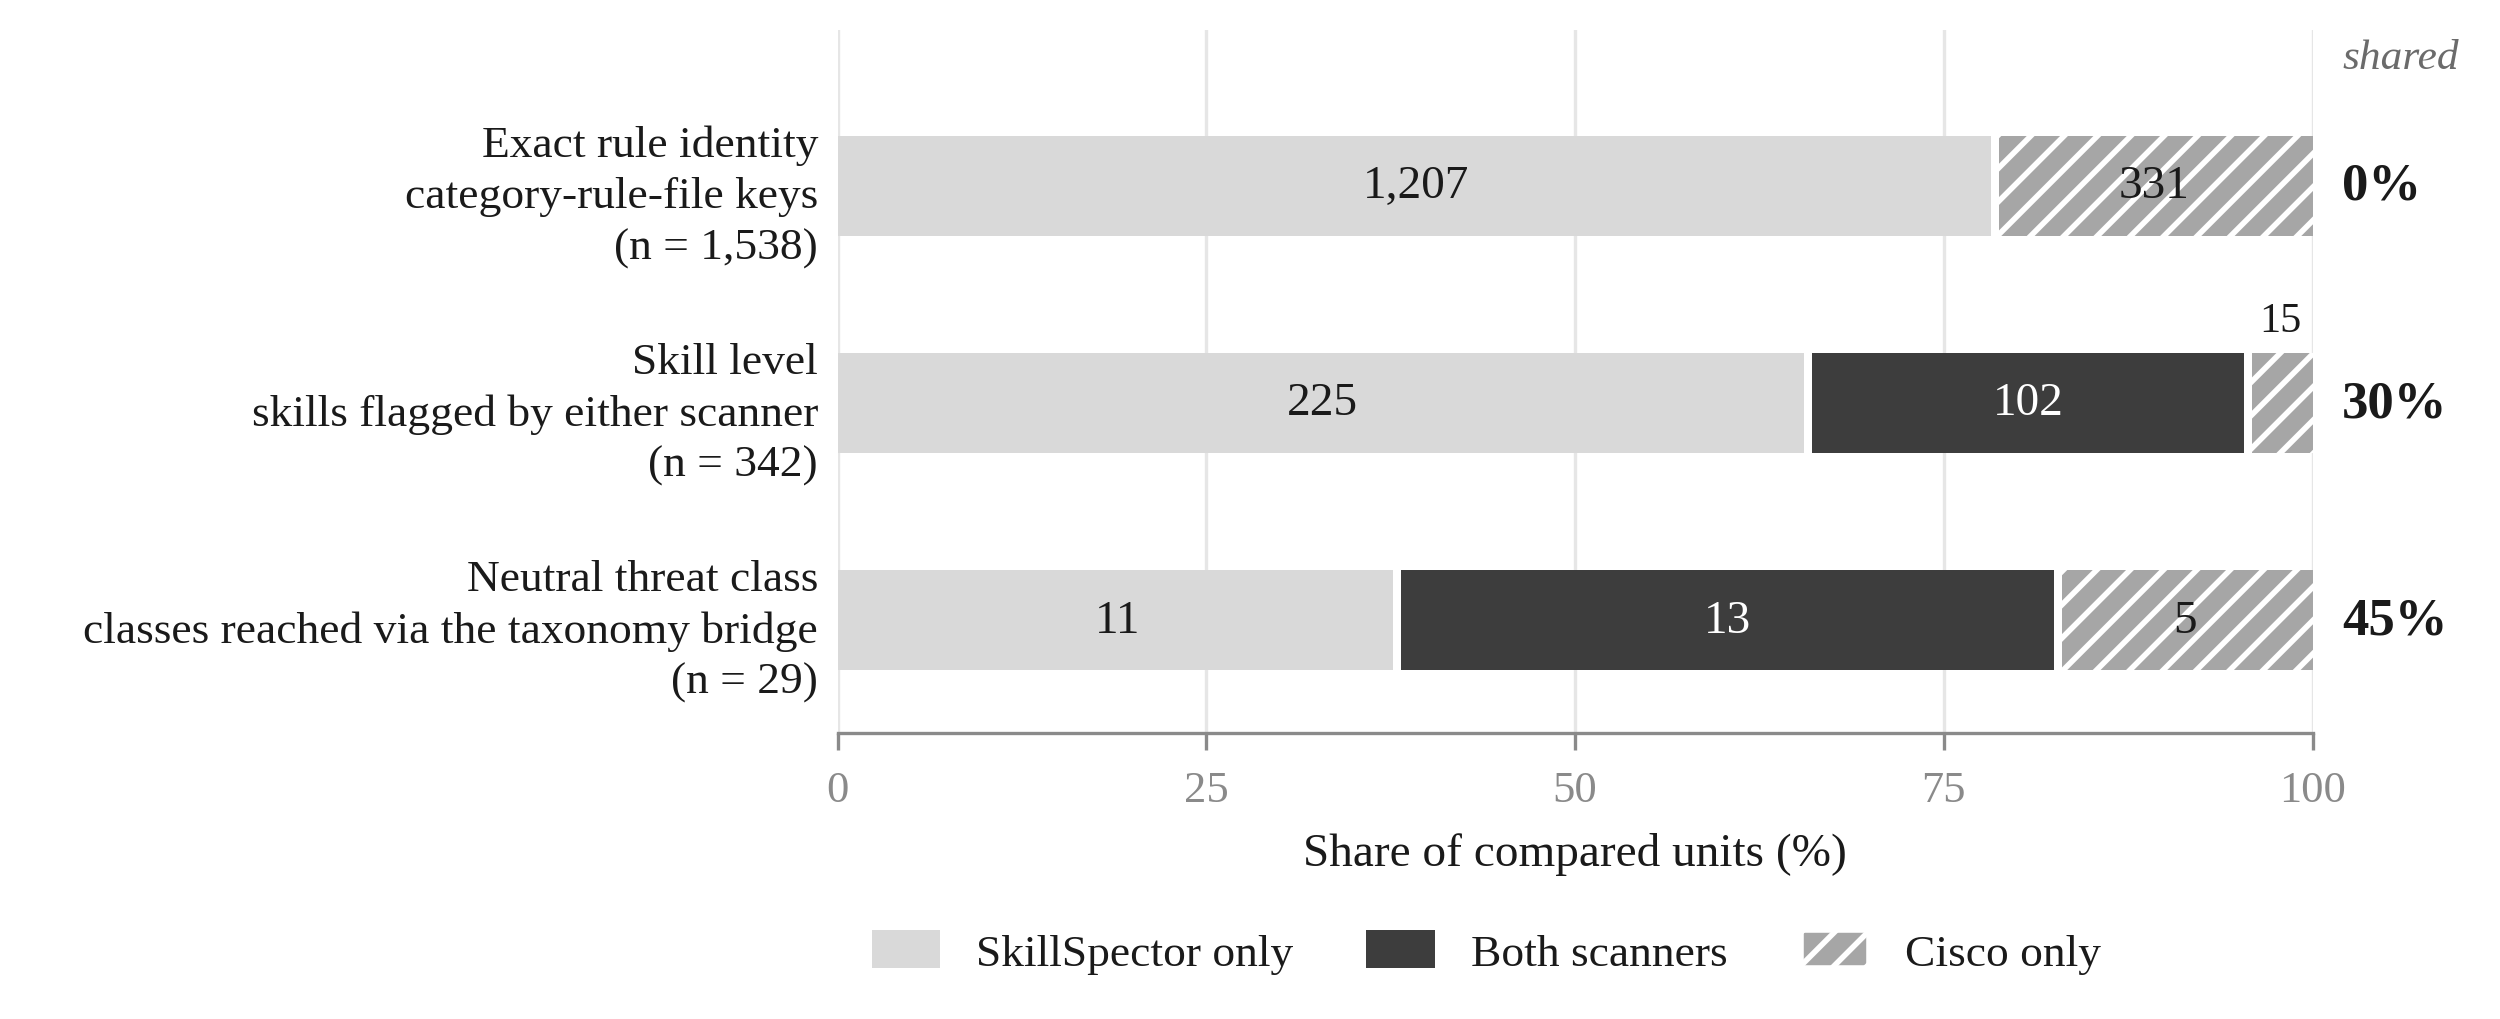
\includegraphics[width=\textwidth]{fig1_agreement.png}
\caption{Scanner agreement at three levels of abstraction. Each bar is
normalized to the units either scanner produced at that level: 1,538 distinct
category-rule-file keys, the 342 skills flagged by at least one scanner (the
remaining 393 of 735 are clean for both), and the 29 neutral threat classes
reached through the taxonomy bridge. Agreement is zero on exact rule identity,
30\% at the skill level and 45\% at the class level; within the 102 jointly
flagged skills the bridge recovers 127 shared skill-class pairs.}
\label{fig:agreement}
\end{figure*}


The taxonomy bridge changes the interpretation of scanner agreement. Although exact scanner vocabularies have no overlap, mapping their rules to reviewed neutral threat classes recovers 127 shared skill-class pairs. The result shows that a meaningful portion of the apparent disagreement is representational: the scanners can identify the same type of risk while naming and structuring it differently.

The same mapping is used to evaluate coverage. We gate the denominator to classes that are reviewed as meaningful targets for skill scanning rather than treating every entry in OWASP or ATLAS as an obligation of a static skill scanner. Under the reviewed denominator, four of twenty mappable classes remain uncovered by both scanners. We therefore report the coverage gap together with the denominator from which it is derived rather than presenting the ratio as framework-independent.

\subsection{Exploratory precision and filtering}

The stratified 50-finding development sample contains 4 true positives and 46 false positives, corresponding to an observed precision of 8.0 percent and a false-positive proportion of 92 percent. This result establishes that raw alert volume is a poor proxy for useful security information and motivates the subsequent filtering experiment.

The initial filtering pipeline suppresses 35 of the 46 false positives without suppressing any of the four labelled true positives. On this development sample, precision therefore rises from 8.0 to 26.7 percent. We treat this as an exploratory and design result rather than as the final estimate of filtering effectiveness: the same labelled sample informed the construction and qualification of the later mitigation pipeline and is therefore excluded from the confirmatory 400-finding test set.

\subsection{Adversarial robustness}

The twelve-skill adversarial suite reveals complementary blind spots. Each scanner detects ten of the twelve malicious skills, but their misses are disjoint. SkillSpector misses a string-reversal obfuscation case and a prescriptive curl-to-shell instruction, whereas Cisco misses a dynamic import and a plain, unobfuscated command-injection case.

The finding is important for deployment because neither scanner is a strict coverage superset of the other. Moreover, one miss requires no obfuscation, showing that adversarial failure is not limited to sophisticated evasion. The thirteen targeted rules derived from these cases probe two broad weaknesses: code-level obfuscation and malicious behaviour expressed directly through natural-language instructions in SKILL.md.

\subsection{Held-out scanner precision}

The independent 400-finding test set confirms that the high false-positive burden observed in the 50-finding development study generalizes. Across the 396 adjudicated findings, 36 are true positives and 360 are false positives, corresponding to an overall false-positive proportion of 90.9\%. Four additional cases remain uncertain and are excluded from the primary binary estimates.

The scanners differ substantially in precision. SkillSpector's 200-unit sample contains 26 true positives, 172 false positives and 2 uncertain findings. Among adjudicated findings, RAW precision is therefore 13.13\%. Cisco contains 10 true positives, 188 false positives and 2 uncertain findings, giving RAW precision of 5.05\%.

These results closely reproduce the direction of the exploratory study, whose 50 findings contained 92\% false positives. The substantially larger held-out sample therefore supports the conclusion that the initial result was not simply an artefact of the development set. At the same time, the difference between SkillSpector and Cisco shows why scanner-specific results are treated as primary rather than pooling the balanced 200/200 test set as though both scanners generated the same underlying population.

\subsection{Deterministic false-positive mitigation}

The strongest reduction in false-positive volume is obtained by O1-BASELINE-OR, the original deterministic policy that suppresses a finding when any contextual component recommends suppression. On SkillSpector, it removes 52 of 172 false positives, an FP-suppression rate of 30.23\%, while suppressing 1 of 26 true positives. True-positive retention is therefore 96.15\%. Precision among retained adjudicated findings increases from 13.13\% under RAW to 17.24\%.

Cisco exhibits a less favourable trade-off. O1-BASELINE-OR removes 41 of 188 false positives, or 21.81\%, but also suppresses 2 of only 10 true positives. TP retention falls to 80.0\%, and retained-finding precision changes only marginally, from 5.05\% to 5.16\%. Thus, although the policy removes substantial alert volume, the cost in genuine findings makes the improvement much less attractive for Cisco.


\begin{figure*}[t]
\centering
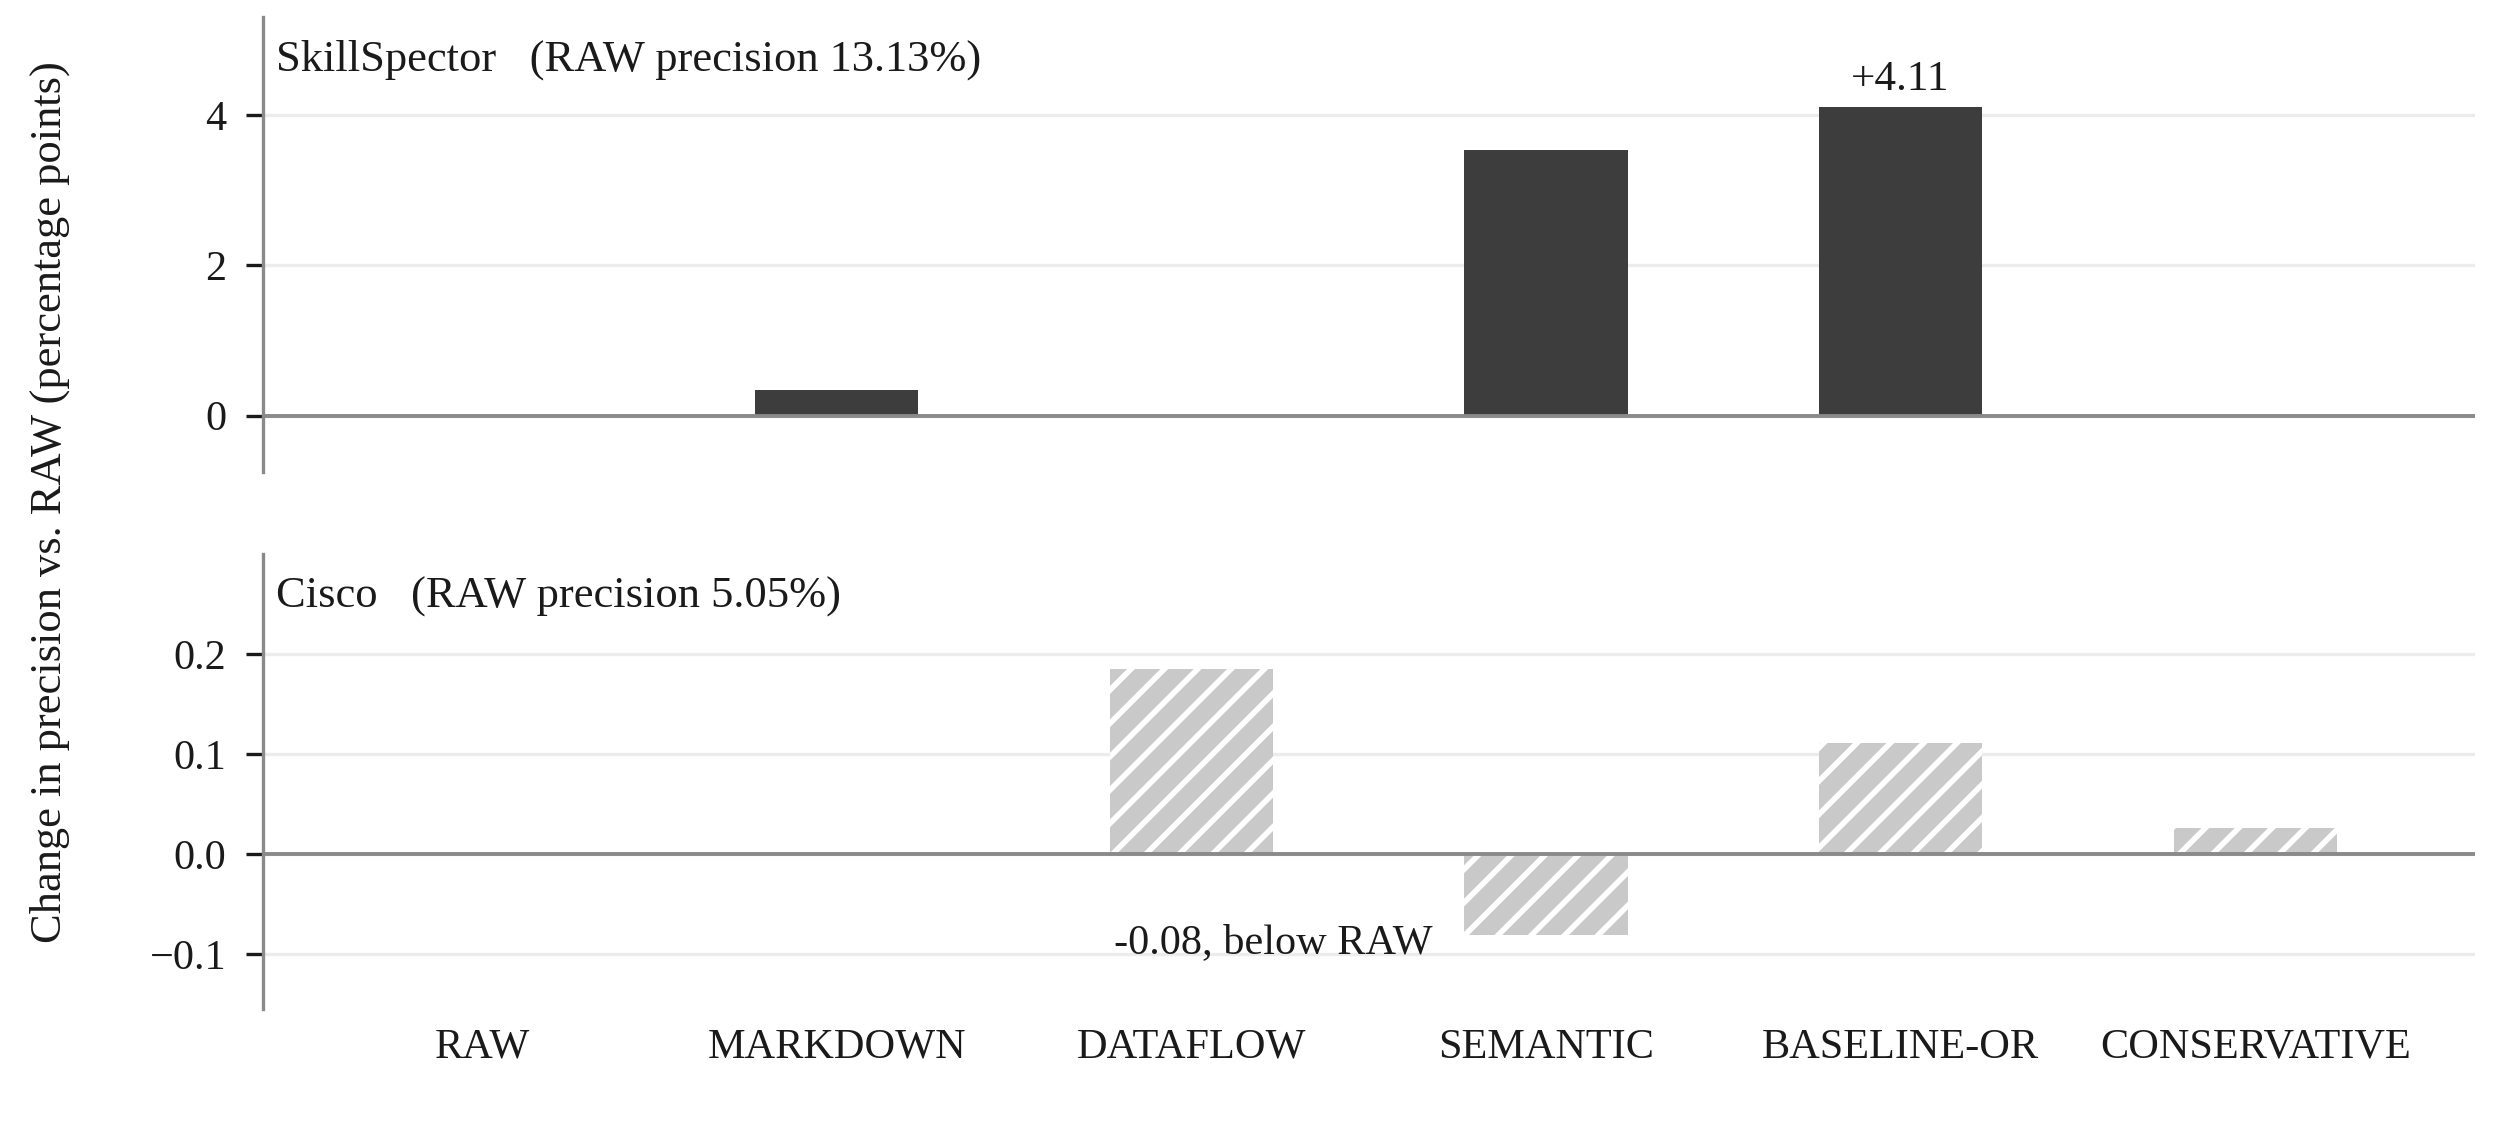
\includegraphics[width=\textwidth]{fig2_mitigation.png}
\caption{Change in precision from deterministic post-processing on the
400-finding held-out test set (396 adjudicated), relative to each scanner's RAW
baseline. The scanners are plotted separately because their RAW baselines
differ by a factor of 2.6 and the Cisco effects are an order of magnitude
smaller, so a shared axis would hide them. Only O1-SEMANTIC and the
O1-BASELINE-OR policy that subsumes it move SkillSpector precision appreciably,
by $+4.11$ points; on Cisco every effect is under a quarter of a point, and
O1-SEMANTIC alone moves precision backwards, from 5.05\% to 4.97\%.}
\label{fig:mitigation}
\end{figure*}


The semantic-context component accounts for most of the suppression produced by the OR policy, while the markdown-context and data-flow components contribute a smaller number of additional false-positive removals. In contrast, O1-CONSERVATIVE preserves all observed true positives but performs almost no filtering: it suppresses no SkillSpector findings and only one Cisco false positive. The held-out experiment therefore reveals a clear operating trade-off. Aggressive deterministic combination can materially reduce scanner noise but may sacrifice genuine findings, whereas strong consensus protects true positives at the cost of almost all filtering utility. Fig.~\ref{fig:mitigation} shows the resulting change in precision for every method and scanner.

\begin{table}[t]
\caption{Held-out performance of every post-processing method on each scanner (400-finding blind test set, 396 adjudicated).}
\label{tab:heldout}
\centering\footnotesize
\setlength{\tabcolsep}{3.5pt}
\begin{tabular}{@{}llrrrr@{}}
\toprule
\textbf{Scanner} & \textbf{Method} & \textbf{Prec.} & \textbf{FP supp.} & \textbf{TP ret.} & \textbf{Abst.} \\
\midrule
SkillSpector & RAW & 13.13\% & 0\% & 100\% & 0\% \\
SkillSpector & Markdown & 13.47\% & 2.91\% & 100\% & 47.5\% \\
SkillSpector & Dataflow & 13.13\% & 0\% & 100\% & 100\% \\
SkillSpector & Semantic & 16.67\% & 27.33\% & 96.15\% & 76.0\% \\
SkillSpector & OR & 17.24\% & 30.23\% & 96.15\% & 0\% \\
SkillSpector & Conservative & 13.13\% & 0\% & 100\% & 0\% \\
\midrule
Cisco & RAW & 5.05\% & 0\% & 100\% & 0\% \\
Cisco & Markdown & 5.05\% & 0\% & 100\% & 52.5\% \\
Cisco & Dataflow & 5.24\% & 3.72\% & 100\% & 90.0\% \\
Cisco & Semantic & 4.97\% & 18.62\% & 80.0\% & 80.5\% \\
Cisco & OR & 5.16\% & 21.81\% & 80.0\% & 0\% \\
Cisco & Conservative & 5.08\% & 0.53\% & 100\% & 0\% \\
\bottomrule
\end{tabular}
\end{table}

\subsection{Native-LLM operational feasibility}

Native LLM-assisted scanner execution is reported as an operational feasibility result rather than an effectiveness comparison. Ten successful SkillSpector SS1 smoke executions required approximately 64.3 minutes in total, averaging 6.43 minutes per skill. A simple extrapolation at the observed rate gives approximately 78.7 hours for SS1 over the 735-skill corpus alone, before adding Cisco LLM or Meta-Analyzer execution.

Ten Cisco CS2 smoke executions also completed successfully, demonstrating that the local integration path was functional, while CS3 was not advanced to a completed evaluation. Because the runtime limitation was identified before final labels were obtained, the confirmatory protocol was amended rather than partially evaluating an LLM configuration over a non-representative subset. We therefore draw no comparative accuracy conclusion from these smoke runs. Their contribution is operational: under the available local hardware and scanner architectures, corpus-scale native-LLM evaluation was not practical within the experimental budget.

These timings were obtained on a Windows 11 host with an Intel Core i9-13900H, approximately 16 GB RAM and integrated Intel Iris Xe graphics while running the local 8B model; they characterize feasibility on the available project hardware rather than a hardware-independent property of the scanners.

\subsection{Statistical analysis}

Finding-level observations are clustered because multiple findings can originate from the same skill or repository. We therefore estimate confidence intervals primarily through skill-clustered bootstrap resampling, with repository-clustered bootstrap used as a sensitivity analysis. Paired method differences are evaluated using multiplicity-preserving paired bootstrap resampling, and McNemar tests are used for paired binary comparisons where appropriate. Cochran's Q and corrected pairwise analyses are used for multi-method comparisons.

For O1-BASELINE-OR, SkillSpector's 30.23\% false-positive suppression has a skill-clustered 95\% bootstrap interval of approximately 21.1\%--39.9\%, while its 96.15\% true-positive retention has an interval of approximately 83.3\%--100\%. Cisco's 21.81\% false-positive suppression has an interval of approximately 13.5\%--30.3\%, while its 80.0\% TP retention has a much wider interval of approximately 54.5\%--100\%, reflecting the small number of true positives in the Cisco sample.

Before labeling, we specified a two-percentage-point TP-retention criterion as a practical safety gate. This is not treated as a formal confidence-interval-based non-inferiority test. O1-BASELINE-OR fails the criterion for both scanners: losing one of 26 SkillSpector true positives corresponds to a 3.85-percentage-point reduction, while losing two of 10 Cisco true positives corresponds to a 20-percentage-point reduction. O1-CONSERVATIVE satisfies the retention criterion because it loses no observed true positives, but its false-positive suppression is negligible. The statistical results therefore reinforce the descriptive conclusion that neither deterministic policy dominates across both objectives.

The methods differ significantly in paired correctness for both scanners (SkillSpector Cochran's Q(5)=212.83, p$\approx$1.25$\times 10^{-33}$; Cisco Q(5)=138.95, p$\approx$3.97$\times 10^{-23}$). In Holm-corrected McNemar comparisons against RAW, O1-BASELINE-OR differs significantly for both SkillSpector ($p_{\mathrm{Holm}}$$\approx$9.76$\times 10^{-11}$) and Cisco ($p_{\mathrm{Holm}}$$\approx$1.03$\times 10^{-7}$). Statistical significance, however, does not imply an acceptable operating point: the OR policy still fails the predeclared TP-retention criterion for both scanners.

\section{Conclusion}

Agent skills combine natural-language instructions, executable artifacts and the ambient authority of the host agent, yet the scanners used to review them have received little independent measurement. Our audit shows that comparing these tools requires more than counting alerts. SkillSpector and Cisco expose different vocabularies and produce no exact category-rule-file agreement, yet a reviewed taxonomy bridge recovers substantial agreement at the underlying threat-class level. The bridge is therefore not merely a presentation device but a necessary measurement instrument.

The audit also exposes two different reliability problems. On naturally occurring public skills, the exploratory labelled sample shows a very high false-positive burden, demonstrating that scanner output cannot be interpreted directly as ground truth. Under adversarial evaluation, the scanners instead exhibit complementary false negatives: both miss malicious cases, and their misses are different. High alert volume and broad rule coverage therefore do not imply either precision or robustness.

The held-out evaluation strengthens the false-positive finding substantially. After excluding the original 50 development findings, the independent 400-finding test set contains 360 false positives among 396 adjudicated cases, a 90.9\% false-positive proportion that closely reproduces the exploratory 92\% result. Raw precision remains low for both tools, at 13.1\% for SkillSpector and 5.1\% for Cisco. Scanner findings should therefore be interpreted as candidates for security review rather than as security ground truth.

Deterministic contextual post-processing can reduce this burden, but the held-out experiment also exposes its limits. The original OR-style policy suppresses 30.2\% of SkillSpector false positives while retaining 96.2\% of its true positives and raises retained-finding precision to 17.2\%. For Cisco, it suppresses 21.8\% of false positives but retains only 80\% of true positives, producing almost no precision improvement. A conservative policy preserves every observed true positive but removes almost no noise. The practical lesson is therefore not that one filtering strategy universally solves scanner false positives, but that suppression policies must be evaluated jointly on noise reduction and security-signal retention and may require scanner-specific operating points.

The attempted native-LLM evaluation adds a complementary operational result. Local LLM-assisted scanner modes could be executed successfully, but measured smoke runtime made a corpus-scale comparison impractical on the available hardware; the confirmatory effectiveness study was therefore restricted, before final labels, to deterministic and fully reproducible post-processing. Taken together with the taxonomy and adversarial results, the study shows that deployed skill scanners are neither interchangeable nor self-validating: they use different vocabularies, exhibit complementary blind spots, generate a large amount of benign alert noise, and respond differently to post-processing. A defensible deployment should therefore preserve provenance, interpret findings through a common threat vocabulary, and treat automated filtering as a measured scanner-specific trade-off rather than as an unquestioned safety layer.

\begin{thebibliography}{99}
\bibitem{ref1} Anthropic, ``Agent Skills,'' GitHub repository. [Online]. Available: \url{https://github.com/anthropics/skills}
\bibitem{ref2} K. Greshake, S. Abdelnabi, S. Mishra, C. Endres, T. Holz, and M. Fritz, ``Not what you've signed up for: Compromising real-world LLM-integrated applications with indirect prompt injection,'' in Proc. 16th ACM Workshop on Artificial Intelligence and Security (AISec '23), 2023, pp. 79-90. arXiv:2302.12173.
\bibitem{ref3} C. Huang, X. Huang, N. P. Tran, and A. Milani Fard, ``Model Context Protocol threat modeling and analyzing vulnerabilities to prompt injection with tool poisoning,'' arXiv:2603.22489, Mar. 2026.
\bibitem{ref4} Y. Guo, P. Liu, W. Ma, Z. Deng, X. Zhu, P. Di, X. Xiao, and S. Wen, ``MCPXKIT: The unified toolkit for analyzing Model Context Protocol security,'' IEEE Trans. Dependable and Secure Computing (accepted). arXiv:2508.12538, Aug. 2025.
\bibitem{ref5} L. Beurer-Kellner, A. Kudrinskii, M. Milanta, K. B. Nielsen, H. Sarkar, and L. Tal, ``ToxicSkills: A study of agent skills supply chain compromise,'' Snyk Security Labs, Feb. 5, 2026. [Online]. Available: \url{https://snyk.io/blog/toxicskills-malicious-ai-agent-skills-clawhub/}
\bibitem{ref6} NVIDIA, ``SkillSpector,'' v2.4.4, commit fd25398. [Online]. Available: \url{https://github.com/NVIDIA/SkillSpector}
\bibitem{ref7} Cisco AI Defense, ``skill-scanner,'' v2.0.13, commit 41fec4a. [Online]. Available: \url{https://github.com/cisco-ai-defense/skill-scanner}
\bibitem{ref8} OWASP GenAI Security Project, ``OWASP Top 10 for Large Language Model Applications 2025.'' [Online]. Available: \url{https://genai.owasp.org/llm-top-10/}
\bibitem{ref9} OWASP GenAI Security Project, ``OWASP Top 10 for Agentic Applications for 2026,'' v2.01, Dec. 9, 2025. [Online]. Available: \url{https://genai.owasp.org/resource/owasp-top-10-for-agentic-applications-for-2026/}
\bibitem{ref10} MITRE, ``ATLAS: Adversarial Threat Landscape for Artificial-Intelligence Systems,'' v5.6.0. [Online]. Available: \url{https://atlas.mitre.org/}
\bibitem{ref11} Y. Hou and Z. Yang, ``SkillSieve: A hierarchical triage framework for detecting malicious AI agent skills,'' arXiv:2604.06550, Apr. 2026.
\bibitem{ref12} Y.-T. Lin and C.-M. Yu, ``PhantomSkill: Malicious code injection in agent skill ecosystems,'' arXiv:2606.19191, Jun. 2026.
\bibitem{ref13} X. Jia, J. Liao, S. Qin, K. Ma, W. Guo, Y. Feng, A. Liu, and Y. Liu, ``Seeing is not screening: Multimodal hidden instruction attacks on agent skill scanners,'' arXiv:2606.18198, Jun. 2026.
\bibitem{ref14} A. Delaitre, B. Stivalet, P. E. Black, V. Okun, A. Ribeiro, and T. S. Cohen, ``SATE V report: Ten years of static analysis tool expositions,'' NIST Special Publication 500-326, Oct. 2018. doi:10.6028/NIST.SP.500-326.
\bibitem{ref15} J. Pellew and F. Raza, ``RealVuln: Benchmarking rule-based, general-purpose LLM, and security-specialized scanners on real-world code,'' arXiv:2604.13764, Apr. 2026.
\bibitem{ref16} Y. Xiong and T. Zhang, ``Sifting the noise: A comparative study of LLM agents in vulnerability false positive filtering,'' arXiv:2601.22952, Jan. 2026.
\bibitem{ref17} MITRE, ``Common Attack Pattern Enumeration and Classification (CAPEC).'' [Online]. Available: \url{https://capec.mitre.org/}
\bibitem{ref18} S. Roy, E. Panaousis, C. Noakes, A. Laszka, S. Panda, and G. Loukas, ``SoK: The MITRE ATT\&CK framework in research and practice,'' arXiv:2304.07411, Apr. 2023.
\bibitem{ref19} A. Al Masoud, A. Anju, M. Arazzi, M. Cihangiroglu, V. K. Kembu, S. Nicolazzo, A. Nocera, Vinod P., and S. Sakthidharan, ``Security in LLM-as-a-Judge: A comprehensive SoK,'' arXiv:2603.29403, Mar. 2026.
\bibitem{ref20} J. D. Norman, M. U. Rivera, and D. A. Hughes, ``Reliability without validity: A systematic, large-scale evaluation of LLM-as-a-judge models across agreement, consistency, and bias,'' arXiv:2606.19544, Jun. 2026.
\bibitem{ref21} A. Sejfia and M. Schafer, ``Practical automated detection of malicious npm packages,'' in Proc. 44th Int. Conf. Software Engineering (ICSE), 2022. arXiv:2202.13953.
\bibitem{ref22} S. Pang, Y. Yao, Z. Jiang, Z. Fan, H. Li, and B. Liu, ``PYPILINE: Malicious PyPI package detection via suspicious API knowledge and agent workflow,'' arXiv:2606.19063, Jun. 2026.
\end{thebibliography}

\end{document}
